\chapter{Multi-objective problems}
In real-world environments, considering a single reachability or shorter path problem might not be sufficient for a given situation.
Indeed, building an optimal strategy satisfying one problem could negatively affect other relevant problems.
For instance, we should be interested in a strategy that does not fail to reach a target with a cost bounded and that however optimises the expected cost to this target.
Moreover, we should also be interested in getting a strategy satisfying at a time many reachability problems, and furthermore, many percentile problems. This chapter will introduce \textit{multi-objective} problems, where we are interested in solving \textit{simultaneously} multiple sub-problems introduced in the previous chapters.
\begin{example}[\textit{Communication between nodes in a wireless sensor network}]\label{main-example}
Consider a wireless sensor network containing three nodes $n_0,\, n_1$ and $n_2$. Assume that $n_0, \, n_1$ and $n_3$ are separated by the same distance, that the sensor $n_0$ has to send messages to $n_2$ at regular intervals and that a wall stands between $n_0$ and $n_2$ (cf. Figure \ref{sensor_net}).
\begin{figure}[h!]
  \centering
  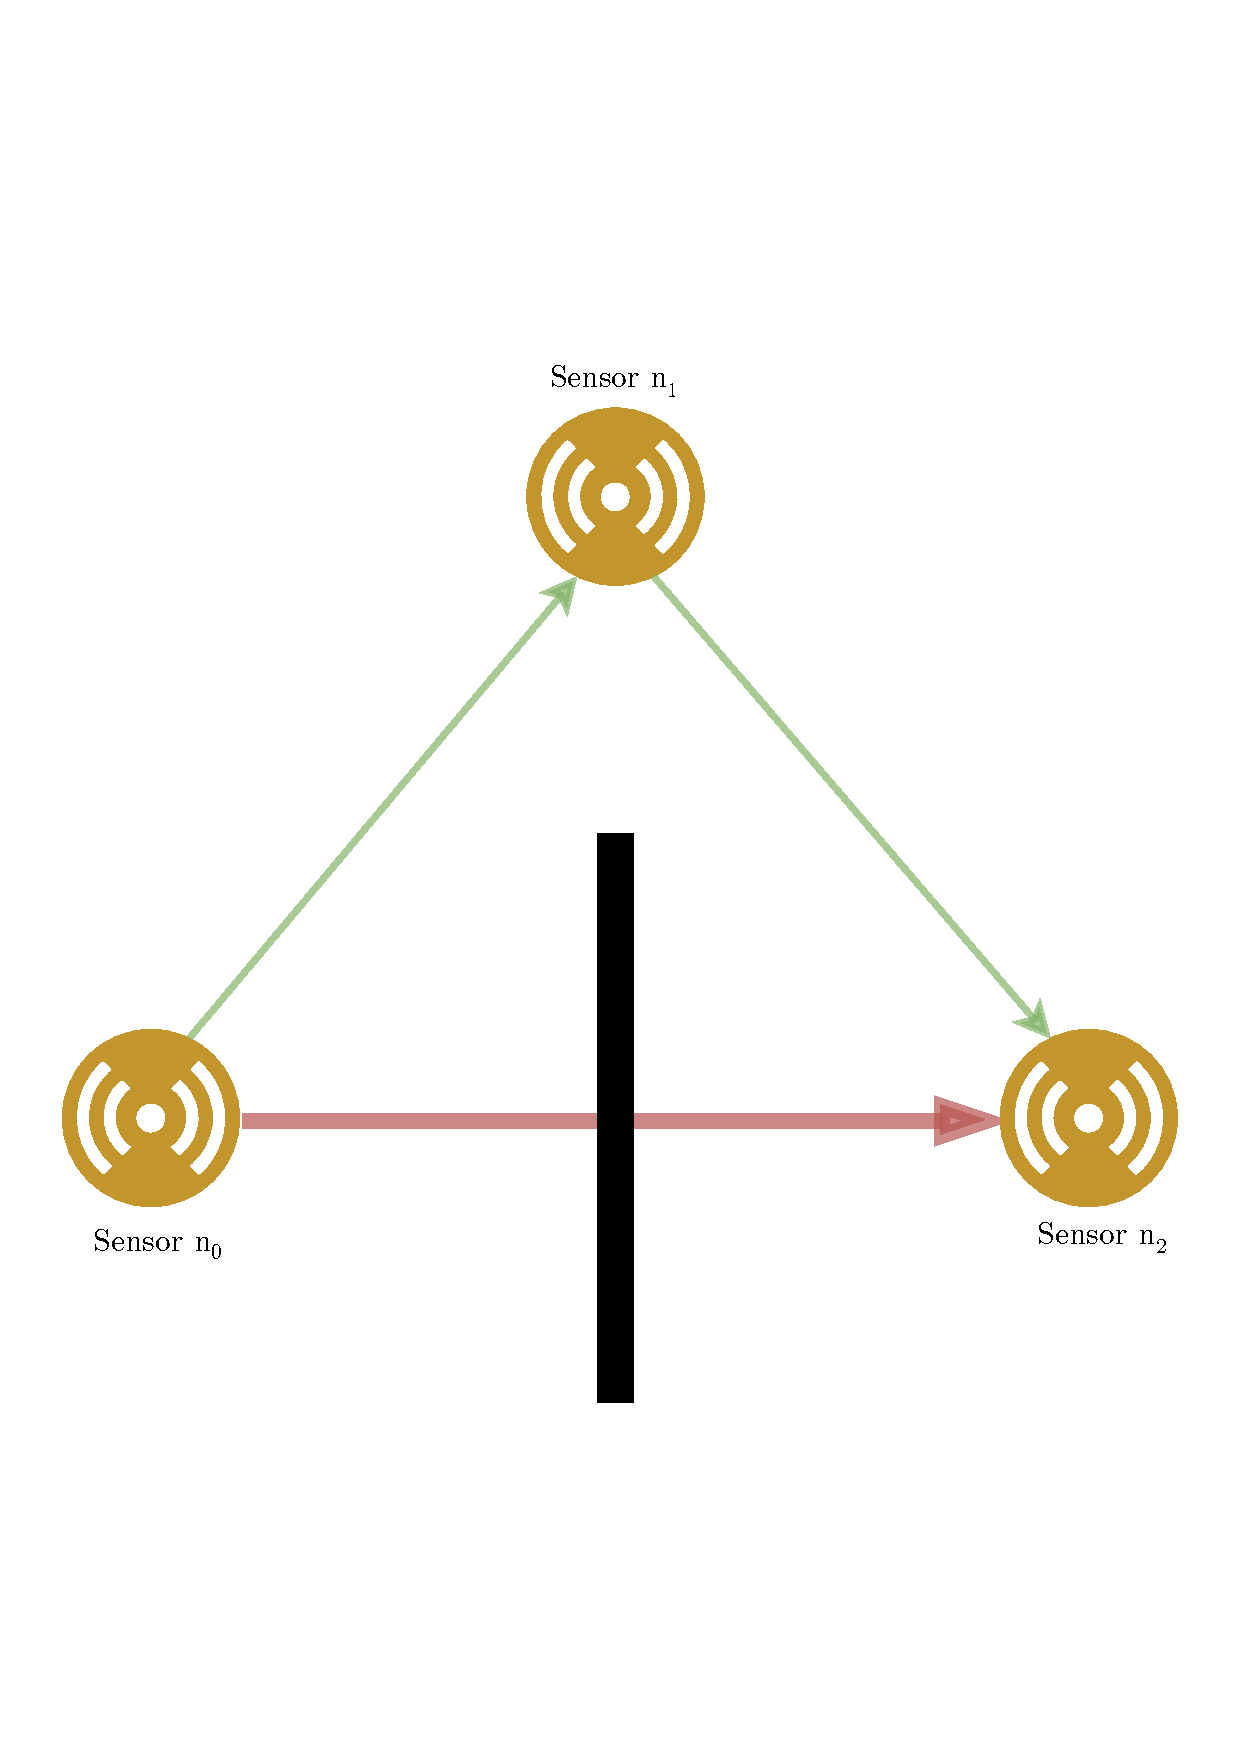
\includegraphics[width=0.7\linewidth]{resources/example3}
  \caption{Communication between three nodes in a wireless sensor network} \label{sensor_net}
\end{figure}
There are two possibilities for $n_0$. First, it can send directly the message to $n_2$. In that case, sending the message is quite quick, but requires more energy that a standard message sending. %(due to the demodulation of a noisy message by $n_2$).
Moreover, this sending has a risk of packet corruption due to the possible noise induced when the signal goes through the wall standing between the two sensors.
The second possibility is to send the message to an intermediate node (i.e., $n_1$). This sending is obviously slower due to the sending in two steps, but requires less energy in total that a direct sending.
In that case, the risk of packet corruption is negligible. \par
This example induces some questions. Firstly, we should be interested by a strategy ensuring a bounded duty cycle for the emitter sensor $n_0$ (i.e., a bounded time for its active state).
Thus, we should be interested by a strategy minimising the expected energy of sending the message while ensuring this duty cycle.
Finally, we should be interested by a strategy offering a good probability to have a bounded duty cycle while having a good probability to minimise the energy used by the sensor to send the message.
\end{example}
\section{Worst case guarantee}
Firstly, we are going to be interested in having a worst case guarantee to reach some states in a Markov decision process, i.e., a guarantee to reach these states with a cost bounded.
To do that, we will approach the problem by considering it as a \textit{shortest path game} problem \cite{DBLP:journals/corr/RandourRS14a}.
\begin{definition}[\textbf{\SPG{} problem}]
  Let $\mathcal{M}$ be an MDP with state space $S$, $s \in S$, $T \subseteq S$, and $l \in \mathbb{N}$.
  The shortest path game problem (\SPG{}, for short) consists in deciding if there exists a strategy $\sigma$ ensuring to reach the subset of target states $T$ from the state $s$ with a cost bounded $l$, i.e.,
  \begin{align*}
    \forall \pi \in Paths^\sigma(s), \, \TS^T(\pi) \leq l.
  \end{align*}
\end{definition}

\begin{theorem}[\textbf{\textit{\SPG{} problem and qualitative cost bounded reachability}}] \label{spg-thm1}
  Let $\mathcal{M}=(S, A, \Delta, w, AP, L)$ be an MDP, $s \in S$, $T \subseteq S$, $l \in \mathbb{N}$, and $\sigma$ be a strategy for $\mathcal{M}$.
  The following two propositions are equivalent:
  \begin{enumerate}[(a)]
    \item $\forall \pi \in Paths^\sigma(s), \, \TS^T(\pi) \leq l$. \label{qsspp1}
    \item $\mathbb{P}_s^\sigma(\Diamond_{\leq \ell}\, T) = 1$. \label{qsspp2}
  \end{enumerate}
\end{theorem}
\begin{proof2}$ $\\
  ($\ref{qsspp1}\implies\ref{qsspp2}$). Assume that for all $\sigma$-path $\pi \in Paths^\sigma(s)$, the truncated sum of this path is lower than or equals $l$, i.e., $\TS^T(\pi)\leq l$.
  We have that $\mathbb{P}_s^\sigma(\Diamond_{\leq \ell}\, T) = \mathbb{P}_s^\sigma(\{ \pi \in Paths(s) \; | \; \TS^T(\pi) \leq \ell \})$. As all $\sigma$-path starting from $s$ have a truncated sum lower than or equals $l$, we have $\{\pi \in Paths^\sigma(s) \; | \; \TS^T(\pi) \leq \ell \} = Paths^\sigma(s)$.
  Then, $\mathbb{P}_s^\sigma(\Diamond_{\leq \ell}\, T) = \mathbb{P}_s^\sigma(Paths(s)) = 1$. \\
  ($\neg \ref{qsspp1} \implies \neg \ref{qsspp2}$). Assume there exists a $\sigma$-path $\pi \in Paths^\sigma(s)$ such that $\TS^T(\pi)>l$. Thus, consider this path $\pi$ and let $\hat{\pi} = s_0\xrightarrow{\alpha_1}\dots \xrightarrow{\alpha_n} s_n \in Pref(\pi)$, where $\alpha_i$ is
  chosen by the strategy $\sigma$ for each $i \in \{1, \dots, n \}$, such that $\sum_{i=1}^n w(\alpha_i) > l$.
  We have $\pi \in Cyl(\hat{\pi})$ and $\mathbb{P}_s^\sigma(Cyl(\hat{\pi})) = \prod_{i=0}^{n-1} \Delta(s_i, s_{i+1}) > 0$.
  We obviously additionally have that $Cyl(\hat{\pi}) \cap \{ \pi \in Paths^\sigma(s) \; | \; \TS^T(\pi) \leq \ell \} = \emptyset$, because %$s_i \not \in T$ for all $i \in \{0, \dots, n\}$ and
  %$\sum_{i=1}^n w(\alpha_i) > l$.
  $\TS^T(\hat{\pi}) > l$.
  Then, we have
   \[\mathbb{P}_s^\sigma(\Diamond_{\leq \ell}\, T) = \mathbb{P}_s^\sigma(\{ \pi \in Paths(s) \; | \; \TS^T \leq \ell \}) \leq 1 - \mathbb{P}_s^\sigma(Cyl(\hat{\pi})) < 1.\]
\end{proof2}
\\

With the theorem \ref{spg-thm1}, it is possible to solve the \SPG{} problem by reduction to the \SSPP{} problem.
However, the \SSPP{} problem is computed in pseudo-polynomial time in $\mathcal{M}$ and in the size of length of $l$, and we want to avoid this class of time complexity.
Here, we consider the MDP as a two players game.
In each step, the system is in state $s$ and the player one chooses an enabled action $\alpha$ of $s$.
Then, the player two chooses the $\alpha$-successor of $s$ leading the worst case in terms of truncated sum.
Thus, we do not consider probabilities for this problem but rather consider the worst case of choosing each action.
Finding an optimal strategy for the player one allowing to reach $T$ with a cost less than or equals $l$
under the choices of the player two solves the \SPG{} problem. \\

We compute the shortest path in this game from $s$ to $T$ by dynamic programming in order to build a strategy solving the \SPG{} problem.
Let $|S| = n$ and $\mathbb{C}: S \times \{0, \dots, n-1 \}$ be a function such that $\mathbb{C}(s, i)$ is the shortest path from $s$ to $T$ in this game after maximum
$i$ playing steps.
Obviously, $\mathbb{C}$ can be represented with a matrix of size $n \times n$.
We have \[\mathbb{C}(s, 0) = \begin{cases}
  0 & \text{if } s \in T\\
  +\infty & \text{else}.
\end{cases}\]
Thus, let $k \in \mathbb{N}$, such that $0 \leq k < n - 1$,
\[
  \mathbb{C}(s,\, k+1) = \min \big[\mathbb{C}(s,\, k),\, \min_{\alpha \in A(s)} \max_{s' \in Succ(s,\alpha)} \big(w(\alpha) + \mathbb{C}(s',\, k)\big)\big].
\]
This recursive definition of $\mathbb{C}$ actually means that the shortest path from $s$ to $T$ in maximum $k+1$ steps corresponds to either the shortest path from $s$ to $T$ in maximum $k$ steps or the minimal weight of choosing an action $\alpha$ plus the shortest path from the worst $\alpha$-successor $s'$ of $s$ to $T$ in maximum $k$ steps.
\begin{figure}[h]
  \centering
  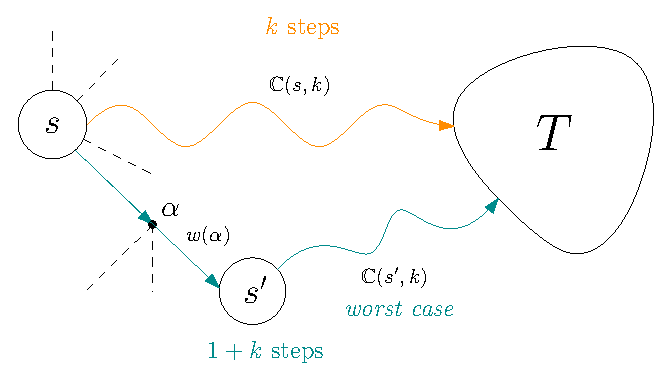
\includegraphics[width=0.6\linewidth]{resources/sp-g}
  \captionsetup{justification=centering}
  \caption{Intuitive representation of  the function $\mathbb{C}$ to solve the \SPG{} problem}
\end{figure}
The minimisation term according to an action in this definition corresponds to the choice of the strategy (i.e., the player one).
The maximisation term in this definition corresponds to the adversary (i.e., the player two), choosing the worst $\alpha$-successor of $s$.
As the weight of each action is strictly positive, the strategy never chooses an action leading to a cycle in this game if it is possible to avoid it.
Then, choosing an action leading to a cycle necessarily yields an infinite truncated sum, and if a strategy satisfying this problem exists, it wins in at most $n - 1$ steps. It is why we only need to consider the $n$ first steps.

\begin{theorem}[\textit{\textbf{Solving the \SPG{} problem}}] The \SPG{} problem can be decided in polynomial time in the size of $\mathcal{M}$ and % with the recursive function $\mathbb{C}$ (and more precisely in $\mathcal{O}(n^2)$ with memoization).
an optimal pure memoryless strategy always exists.% and can also be built in $\mathcal{O}(n^2)$.
\end{theorem}

By dynamic programming, we can determine all values of $\mathbb{C}$ for all entries $(s, i) \in S \times \{0, \dots, n-1\}$ with a time complexity in $\mathcal{O}(n^2)$.
Let $s$ be a state of the MDP. By definition of $\mathbb{C}$, we have $\mathbb{C}(s,\, k + 1) \leq \mathbb{C}(s,\, k)$, for all $k \in \mathbb{N}$ such that $0 \leq k < n-1$.
Then, we have $\mathbb{C}(s, \, n-1) = \min_{k} \mathbb{C}(s, \, k)$, and
a strategy satisfying the \SPG{} problem for $s \in S$ exists if and only if $\mathbb{C}(s,\, n-1) \leq l$.
Furthermore, we can build this pure memoryless strategy as follows:
\[
  \sigma : S \rightarrow A, \; s \mapsto \arg \min_{\alpha \in A(s)} \big[ \max_{s' \in Succ(s, \alpha)} \big(w(\alpha) + \mathbb{C}(s',\, n - 1) \big) \big].
\]
The key idea behind this definition is that $\sigma$ will choose the action minimising the weight of the enabled actions plus the smallest cost to reach $T$ in this game from the worst successor, chosen by the player two.

\begin{remark}[\textit{\SPG{} problem and PRCTL model checking}]
  Let $\mathcal{M}=(S, A, \Delta, w, AP, L)$ be an MDP, $s \in S$, $l \in \mathbb{N}$, and $\Phi$ be a PRCTL state formula over $AP$,
  verify $s \models \mathcal{P}^{\max}_{=1}(\Diamond_{\leq \ell}\, \Phi)$ is equivalent to solve the \SPG{} problem for the state $s$, the cost threshold $l$ and the subset of target states $Sat(\Phi)$.
\end{remark}

\begin{example}[\textit{\SPG{} problem in the wireless sensor network}] \label{spg-example}
Get back to Example \ref{main-example}.
For this example, we will only consider the time dimension to model the situation.
We focus on the behaviour of the node $n_0$  (cf. Figure \ref{sensor_net_mdp}).
When $n_0$ becomes active, it has to send a message to $n_2$. We assume here that a standard message sending takes $2$ \textit{mili seconds} ($ms$). If $n_0$ decides to send the message passing by $n_1$, it must wait to receive an acknowledgement of the message sent from $n_1$ to $n_2$. We assume that an acknowledgement message take $2$ $ms$ to be received.
Thus, we have that $n_0$ sends the message to $n_1$ ($2$ $ms$), then $n_1$ sends the message to $n_2$ ($2$ $ms$). When $n_2$ receives the message, it sends an acknowledgement to $n_1$ ($2$ $ms$) and $n_1$ sends an acknowledgement to $n_0$ ($2$ $ms$).
Then, after that $n_0$ has sent the message to $n_1$, he waits $6$ $ms$ the acknowledgement from $n_1$ and go to sleep during $10$ $ms$ after that. If $n_0$ decides to directly send a message to $n_2$, then $n_2$ sends the message and waits $2$ $ms$ the acknowledgement.
Due to the possible packet corruption, $n_2$ does not receive the acknowledgement with a probability $\frac{1}{8}$. In that case, it has to try sending the message again.
Else, it goes to sleep during $10$ $ms$.
\begin{figure}[h]
  \centering
  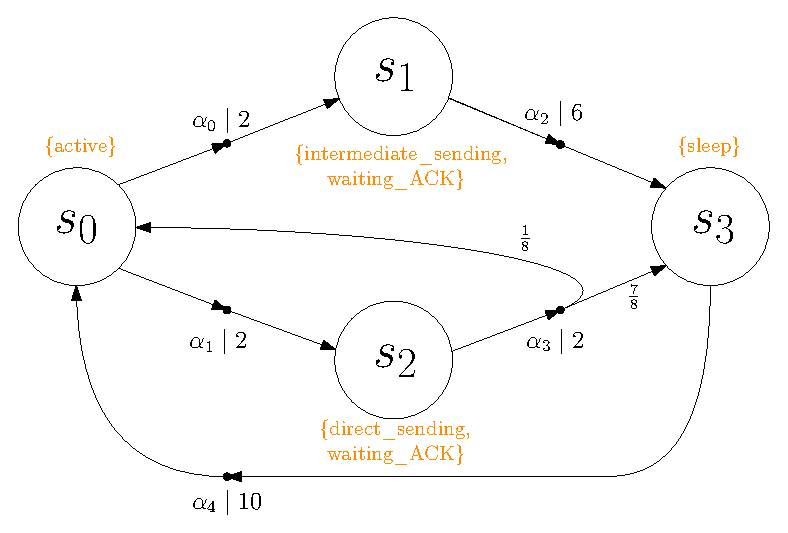
\includegraphics[width=0.6\linewidth]{resources/example3.eps}
  \captionsetup{justification=centering}
  \caption{MDP representing the behaviour of the node $n_0$, according to the situation of Figure \ref{sensor_net} from Example \ref{main-example}}\label{sensor_net_mdp}
\end{figure}

Assume we want to ensure a duty cycle of $12$ $ms$ for the node $n_0$. Then, let $\mathcal{M}=(S, A, \Delta, w, AP, L)$ be the MDP of Figure \ref{sensor_net_mdp}, we want to solve the following \SPG{} problem:
\[
  s_0 \overset{?}{\models} \, \mathcal{P}^{\max}_{=1}(\Diamond_{\leq 12} \; \textit{sleep}).
\]
To solve this problem, we will recursively compute $\mathbb{C}$ for all $s \in S$ from $k=0$ to $k=3$:
\begin{minipage}{0.5\linewidth}
    \begin{itemize}
      \item[$k=0$] \begin{itemize}
[label=\raisebox{0.25ex}{\tiny$\bullet$}]        \item $\mathbb{C}(s_0, 0) = \mathbb{C}(s_1, 0) = \mathbb{C}(s_2, 0) = +\infty$
        \item $\mathbb{C}(s_3, 0) = 0$
      \end{itemize}
      \item[$k=1$]
        \begin{itemize}
[label=\raisebox{0.25ex}{\tiny$\bullet$}]          \item $\mathbb{C}(s_0, 1) = +\infty$
          \item $\mathbb{C}(s_1, 1) = 6 + 0 = 6$
          \item $\mathbb{C}(s_2, 1) = 2 + \infty = +\infty$
        \end{itemize}
      \item[$k=2$]
        \begin{itemize}
[label=\raisebox{0.25ex}{\tiny$\bullet$}]          \item $\mathbb{C}(s_0, 2) = 2 + 6 = 8$
        \end{itemize}
      \item[$k=3$]
        \begin{itemize}
[label=\raisebox{0.25ex}{\tiny$\bullet$}]          \item $\mathbb{C}(s_2, 3) = 2 + 8 = 10$
        \end{itemize}
    \end{itemize}
\end{minipage}
\begin{minipage}{0.5\linewidth}
\centering
\begin{tabular}{l|llll}
$S$ & $k=0$     & $k=1$     & $k=2$     & $k=3$ \\ \hline
$s_0$  & $+\infty$ & $+\infty$ & 8         & 8     \\
$s_1$  & $+\infty$ & 6         & 6         & 6     \\
$s_2$  & $+\infty$ & $+\infty$ & $+\infty$ & 10    \\
$s_3$  & 0         & 0         & 0         & 0
\end{tabular}
\captionsetup{justification=centering}
\captionof{table}{Computing $\mathbb{C}$ by dynamic programming}
\end{minipage}
\\$ $\\$ $\\
The result $\mathbb{C}(s_2,3)=10$ is interesting. It means that the player one firstly chooses the action $\alpha_3$ (with a weight of $2$).
Then, the player two chooses worst case, i.e., the transition $s_2 \xrightarrow{\alpha_3}s_0$, and the player one next chooses the action surely leading $s_0$ to $s_3$ with a minimal cost (i.e., $\mathbb{C}(s_0, 2)=8$ with $s_0\xrightarrow{\alpha_0}s_1\xrightarrow{\alpha_2}s_3$).
\par As $\mathbb{C}(s_0,\, 3) \leq 12$, the duty cycle is ensured by the strategy built with $\mathbb{C}$, and we have $s_0 \models \mathcal{P}^{\max}_{=1}(\Diamond_{\leq 12}\; \textit{sleep})$.
With this strategy, the sensor $n_0$ will always choose to send the message via $n_1$.
This ensures a duty cycle of $8$ $ms$, but it is possible to have a better expected time to reach the \textit{sleep} state (e.g., with a memory strategy).
Thus, the next type of strategy that we will study is strategies offering a good expected cost-to-target while ensuring to reach this target with a cost bounded.
\end{example}

\section{Good expectation under a worst case}
We study now strategies ensuring simultaneously a worst case guarantee (cf. previous section) and a good expected cost-to-target in a Markov decision process \cite{DBLP:journals/corr/RandourRS14a, DBLP:journals/iandc/BruyereFRR17}.
$ $ \\ $ $ \\
\begin{definition}[\textbf{\SSPWE{} problem}]
    Let $\mathcal{M}=(S, A, \Delta, w, AP, L)$, be an MDP, $s \in S$, $T \subseteq S$, and $\ell_1, \ell_2 \in \mathbb{N}$.
    The \textit{stochastic shortest path worst case expectation} problem (\SSPWE{}, for short) consists in deciding if there exists a strategy $\sigma$ such that:
    \begin{itemize}
      \item $\forall \pi \in Paths^\sigma(s), \; TS^T(\pi) \leq \ell_1$.
      \item $\mathbb{E}_s^\sigma(\TS^T) \leq \ell_2$.
    \end{itemize}
\end{definition}

The \SSPWE{} problem is thus a \textit{multi-objective} problem: indeed, we want actually to solve simultaneously the \SPG{} problem and the \SSPE{} problem.
As a reminder, in the previous section we have replaced the probabilities by an adversarial choice to handle the guarantee to reach a set of target states respecting a worst case.
Here, we will combine this approach with taking into account probabilities for the expected cost-to-target part.
Although the \SSPE{} and the \SPG{} problems can both be decided in polynomial time, the \SSPWE{} is more complex due to the strategy having to satisfy both problems at the same time.
Before introducing an algorithm able to solve the problem, we first define the notion of \textit{attractor}.

\begin{definition}[\textbf{Attractor of a set of target states in an MDP}]
  Let $\mathcal{M}$ be an MDP with state space $S$ and $T \subseteq S$. The set of \textit{attractors} of $T$ is the set of states reaching $T$ with a maximum probability one, i.e., the set $\{ s \in S \; | \; \mathbb{P}^{\max}_s (\Diamond T) = 1 \}$.
\end{definition}

Let $\mathcal{M}=(S, A, \Delta, w, AP, L)$ be an MDP, the \SSPWE{} problem for $\mathcal{M}$, the state $s \in S$, the subset of target states $T \subseteq S$, and the cost thresholds $\ell_1, \ell_2 \in \mathbb{N}$ can be solved with the following algorithm:

\begin{center}
  \hrule height.8pt depth0pt \kern2pt% \@fs@pre for \@fs@ruled
  \captionof{algorithm}{Solving the \SSPWE{} problem}\label{sspwe-algo}
  \vspace{-.02\linewidth}
  \offinterlineskip\hrulefill
\begin{enumerate}
  \item We compute the unfolding of $\mathcal{M}$ from $s$ up to the cost threshold $\ell_1$, i.e., $\mathcal{M}_{\ell_1}$ with state space $S_{\ell_1}$.
  %\item We compute $\mathbb{A}: S \times \{0, \dots, \ell_1\} \cup \{\bot\} \rightarrow A$, for each state of $S_{\ell_1}$, yielding the set of \textit{safe actions} allowing to surely go to a successor being in the set of attractors of $T_{\ell_1} = \{ (s, v) \in S_{\ell_1} \; | \; s \in T \, \wedge \, v \leq \ell_1 \}$.
  \item Then, we compute the set of \textit{safe actions} allowing each state in $S_{\ell_1}$ to surely go to a successor being in the set of attractors of
  $T_{\ell_1} = \{ (s, v) \in S_{\ell_1} \; | \; s \in T \, \wedge \, v \leq \ell_1 \}$.
  More formally, we compute \[\mathbb{A}: S_{\ell_1} \rightarrow 2^A, \, (s, v) \mapsto \{ \alpha \in A(s) \; | \; \forall (s', v') \in Succ((s, v), \, \alpha), \, \mathbb{P}^{\max}_{(s', v')}(\Diamond T_{\ell_1}) = 1 \}\]
  for all states $(s, v) \in S_{\ell_1}$. Thus, for each state $(s, v) \in S_{\ell_1}$, $\mathbb{A}(s, v)$
  is the set of actions $\alpha \in A(s)$ ensuring to reach $T_{\ell_1}$ from $(s, v)$ regardless of the evolution of $\mathcal{M}_{\ell_1}$ by the uncertainty associated with the probabilities.
  \item Next, we compute $\mathcal{M}^\mathbb{A}_{\ell_1}$, the unfolding of $\mathcal{M}$ up to $\ell_1$ restricted by the set of attractors of $T_{\ell_1}$. The key idea is that we remove the states $(s, v)$ such that $\mathbb{A}(s, v) = \emptyset$ from $\mathcal{M}_{\ell_1}$. More formally,
  we define $\mathcal{M}^\mathbb{A}_{\ell_1} = (S^\mathbb{A}_{\ell_1}, \mathbb{A}^*, \Delta^*_{\ell_1}, w, AP, L_{\ell_1})$ as follows:
  \begin{itemize}
    \item $S^\mathbb{A}_{\ell_1} = \{ (s, v) \in S_{\ell_1} \; | \; \mathbb{A}(s, v) \neq \emptyset \, \vee \, (s, v) \in T_{\ell_1} \}$,
    \item $\mathbb{A}$ is the set of action of this unfolding such that, for all action $\alpha \in A$, $\alpha \in \mathbb{A}^*$, and the set of enabled actions of each state $(s, v) \in S^\mathbb{A}_{\ell_1}$ is given by %$\mathbb{A}(s, v)$ if $\mathbb{A}(s, v) \neq \emptyset$ and a singleton containing an arbitrary action $\alpha \in A(s)$ else,
    \[
      \mathbb{A}^*(s, v) = \begin{cases}
        \mathbb{A}(s, v) & \text{if } \mathbb{A}(s, v) \neq \emptyset, \, \\
        \{\alpha\}, \; \text{where } \alpha \in A(s) & \text{else},
      \end{cases}
    \]
    \item $\Delta^*_{\ell_1}$ is defined as for the classical unfolding $\mathcal{M}_{\ell_1}$, except for $(s, v)$ such that $\mathbb{A}(s, v) = \emptyset$, where $\Delta^*_{\ell_1}((s, v),\, (s, v)) = 1$ and $\Delta^*_{\ell_1}((s, v), \, (s', v')) = 0$ if $(s', v') \neq (s, v)$.
    \item $w, \, AP, \, L_{\ell_1}$ are defined as for the classical unfolding $\mathcal{M}_{\ell_1}$.
  \end{itemize}
  Note that we define $\mathbb{A}^*$ and $\Delta_{\ell_1}^*$ this way because we must handle the case of $(s, v) \in T_{\ell_1}$ and $\mathbb{A}(s, v) = \emptyset$.
  \item Finally, we solve the \SSPE{} problem in $\mathcal{M}^\mathbb{A}_{\ell_1}$ for the state $(s, 0)$, the subset of target states $T_{\ell_1}$, and the cost threshold $\ell_2$.
\end{enumerate}
$ $\\
\kern2pt\hrule\relax% \@fs@post for \@fs@ruled
\end{center}
\par
Let $(s, v) \in S_{\ell_1}$, the set of safe actions of $(s, v)$, i.e., $\mathbb{A}(s, v)$, can be computed recursively
% with the function $\mathbb{A}_i$, for $i \in \mathbb{N}$, %corresponding to the set of actions ensuring to reach a \textit{safe state} in $i$ steps (i.e., a state in the set of attractors of $T_{\ell_1}$),
%that is defined
as follows:
\[
  \mathbb{A}_0(s, v) = \begin{cases}
    A(s) & \text{if }v \leq \ell_1,\\
    \emptyset & \text{else},
  \end{cases}
\]
then, let $i \in \mathbb{N}$, assume that $\mathbb{A}_i$ has already been computed,
\[
  \mathbb{A}_{i+1}(s, v) = \{ \alpha \in \mathbb{A}_i(s, v) \; | \;
    \forall (s', v') \in Succ( (s, v), \alpha ) \setminus T_{\ell_1}, \; \mathbb{A}_i(s', v') \neq \emptyset \}.
\]
%The key idea behind this definition is that
%$\mathbb{A}_i(s,v)$ is the set of enabled actions of $(s, v)$ ensuring to not reach a \textit{bad state} in at most $i$ transitions.
The key idea behind this definition of $\mathbb{A}_i$ is that we inductively disable the unsafe enabled actions of all states.
We consider that a state that has no more enabled action is a \textit{bad state}.
At the initialisation, i.e., at $i=0$, all enabled actions of each state are safe except if the current cost of a state has exceeded the threshold $\ell_1$. In that case, this state is a bad state.
%Then, we inductively consider the successors  of $(s, v)$ reachable in $i$ steps from the current state $(s, v)$ and inductively remove the enabled actions of $(s, v)$ ensuring to reach a bad states from one of these successors, in at most $i$ steps.
%Then, we inductively increase the scope of successors considered up to a \textit{bad state}, i.e., a state exceeding the cost $\ell_1$. Each action
By induction, at each step and for each state $(s, v)$,
%By induction, at the step $i$,
we disable the actions $\alpha$
%of each state
that risk to lead $(s, v)$ to one of its $\alpha$-successor considered as a bad state.% in at most $i$ transitions.
\begin{figure}[h]
  \begin{minipage}{0.5\linewidth}
    \centering
    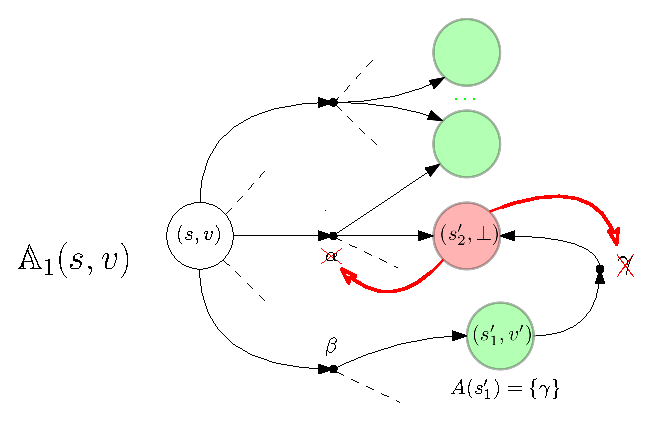
\includegraphics[width=0.9\linewidth]{resources/attractor}
  \end{minipage}
  \begin{minipage}{0.5\linewidth}
    \centering
    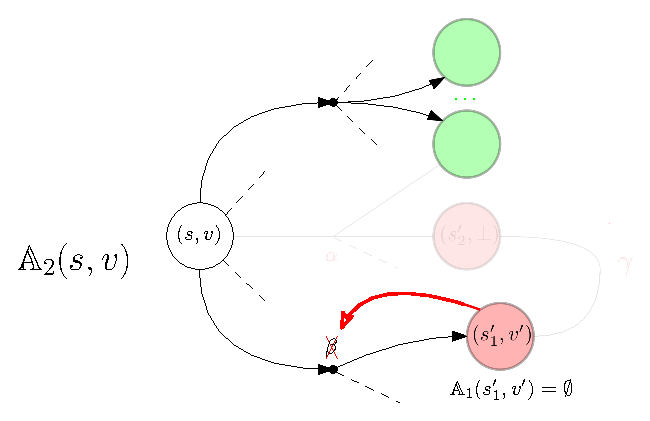
\includegraphics[width=0.9\linewidth]{resources/attractor2}
  \end{minipage}
  \caption{Intuition of the recursive computation of $\mathbb{A}$}
\end{figure}

The way we compute $\mathbb{A}$ is actually the same
as when we compute the largest set $S_{=1} = \{ s \in S \; | \; \mathbb{P}^{\max}_s(\Diamond T) = 1 \}$ (cf. algorithm \ref{prMax1} from Appendix \ref{LP-app}).
Computing $\mathbb{A}$ this way particularises the algorithm \ref{prMax1} for $\mathcal{M}_{\ell_1}$ to only keep the actions leading to attractors of $T_{\ell_1}$, in order to build $\mathcal{M}^\mathbb{A}_{\ell_1}$ and solve the \SSPE{} problem in it.

\begin{theorem}[\textbf{\textit{Solving the \SSPWE{} problem}}]
  The \SSPWE{} problem can be decided in pseudo-polynomial time in the size of $\mathcal{M}$ and in the size of the length of $\ell_1$.
  Pure pseudo-polynomial memory strategies are sufficient and in general necessary, and strategies satisfying this problem can be built in pseudo-polynomial time in the size of $\mathcal{M}$ and in the size of the length of $\ell_1$.
\end{theorem}

By definition, the size of the set $\mathbb{A}_i$ is decreasing with $i$, i.e., for all $i \in \mathbb{N}$,
\[
  | \mathbb{A}_i | \geq | \mathbb{A}_{i+1} |.
\]
By construction, the underlying graph of the unfolding of $\mathcal{M}$ up to $\ell_1$ is a directed acyclic graph (i.e., a DAG). Moreover, the weight of each action is a strictly positive integer. Then, there is no cycle in $\mathcal{M}_{\ell_1}$ and each state reach $T_{\ell_1}$ in at most $\ell_1$ transitions (this worst case corresponds to the case of $w(\alpha)=1$ for all $\alpha \in A$).
The time complexity of the construction of $\mathbb{A}$ is thus polynomial in the size of $\mathcal{M}_{\ell_1}$ (more precisely in $\mathcal{O}(\ell_1 \times |S_{\ell_1}|) = \mathcal{O}(\ell_1^2 \times |S|)$), and is thus pseudo-polynomial in the size of $\mathcal{M}$ and in the size of the length of $\ell_1$. Then, as solving the \SSPE{} problem in $\mathcal{M}^\mathbb{A}_{\ell_1}$ is polynomial in the size of $\mathcal{M}^\mathbb{A}_{\ell_1}$,
the entire algorithm presented to solve this problem is pseudo-polynomial in the size of $\mathcal{M}$ and in the size of the length of $\ell_1$.
Furthermore, as the strategy solving the \SSPE{} problem in $\mathcal{M}_{\ell_1}^\mathbb{A}$ is memoryless in $\mathcal{M}_{\ell_1}^\mathbb{A}$, it requires pseudo-polynomial memory in $\mathcal{M}$ (intuitively, the strategy has $\ell_1 + 1$ modes).

\begin{example}[\textit{\SSPWE{} problem in the wireless sensor network}]
  Again, get back to Example \ref{main-example}.
  We consider the MDP $\mathcal{M}$ of Figure \ref{sensor_net_mdp}. As in Example \ref{spg-example}, we are interested by a strategy ensuring a duty cycle of $12$ $ms$ for the node $n_0$, but at the same time ensuring a minimal expected time to reach the \textit{sleep} state, allowing it to go to sleep as soon as possible.
  Assume that we are interested by the following \SSPWE{} problem:
  \[
    ?\exists \sigma \; \;  \mathbb{P}^\sigma_{s_0}(\Diamond \{s_2\}) \leq 12 \; \wedge \; \mathbb{E}^\sigma_{s_0}(\TS^{\{s_2\}}) \leq 6,
  \]
  where $6$ $ms$ is half the time of the duty cycle that we want to ensure. First, we begin by unfolding $\mathcal{M}$ from $s_0$ up to the cost threshold $12$ (cf. Figure \ref{unfolding-sspwe}), yielding the MDP $\mathcal{M}_{\ell_1}$.
  \begin{figure}[h]
    \centering
    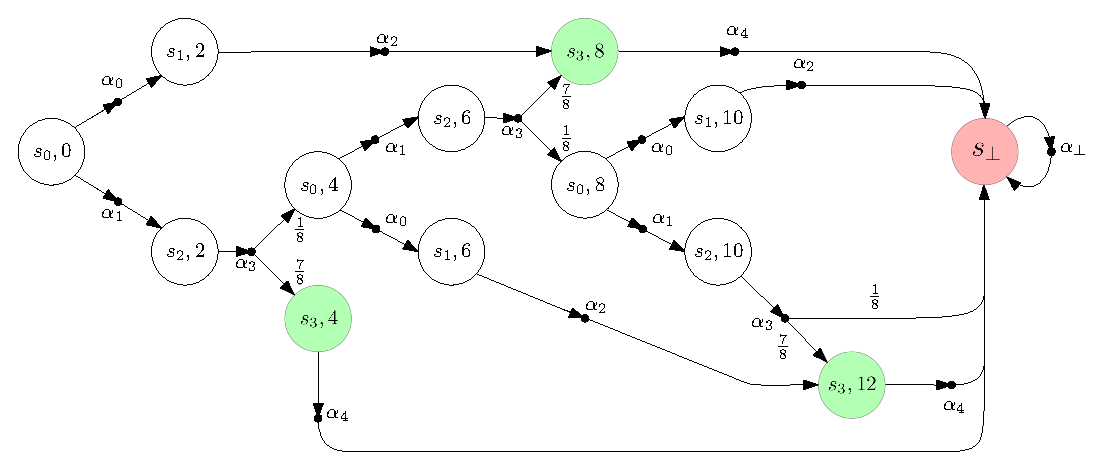
\includegraphics[width=0.9\linewidth]{resources/main-example-unfolding}
    \captionsetup{justification=centering}
    \caption{Unfolding of $\mathcal{M}$ (cf. Figure \ref{sensor_net_mdp}) from $s_0$ (i.e., from the active state) up to $12$ $ms$}
    \label{unfolding-sspwe}
  \end{figure}
  \begin{table}[h]
  \centering
\begin{tabular}{l|cccccc}
$S_{12}$          & \multicolumn{1}{l}{$i=0$} & \multicolumn{1}{l}{$i=1$}                                  & \multicolumn{1}{l}{$i=2$}  & \multicolumn{1}{l}{$i=3$}  & \multicolumn{1}{l}{$i=4$} & \multicolumn{1}{l}{$i=5$} \\ \hline
$s_0, \, 0$  & $\alpha_0, \alpha_1$      & $\alpha_0, \alpha_1$                                       & $\alpha_0, \alpha_1$       & $\alpha_0, \alpha_1$       & $\alpha_0, \alpha_1$      & $\alpha_0, \alpha_1$      \\
$s_1, \, 2$  & $\alpha_2$                & $\alpha_2$                                                 & $\alpha_2$                 & $\alpha_2$                 & $\alpha_2$                & $\alpha_2$                \\
$s_2, \, 2$  & $\alpha_3$                & $\alpha_3$                                                 & $\alpha_3$                 & $\alpha_3$                 & $\alpha_3$                & $\alpha_3$                \\
$s_0, \, 4$  & $\alpha_1, \alpha_0$      & $\alpha_1, \alpha_0$                                       & $\alpha_1, \alpha_0$       & $\alpha_1, \alpha_0$       & ${\color{red}\alpha_0}$   & $\alpha_0$                \\
$s_3, \, 4$  & $\alpha_4$                & ${\color{red}\varnothing}$                                 & $\varnothing$              & $\varnothing$              & $\varnothing$             & $\varnothing$             \\
$s_1, \, 6$  & $\alpha_2$                & $\alpha_2$                                                 & $\alpha_2$                 & $\alpha_2$                 & $\alpha_2$                & $\alpha_2$                \\
$s_2, \, 6$  & $\alpha_3$                & $\alpha_3$                                                 & $\alpha_3$                 & ${\color{red}\varnothing}$ & $\varnothing$             & $\varnothing$             \\
$s_0, \, 8$  & $\alpha_0, \alpha_1$      & $\alpha_0, \alpha_1$                                       & ${\color{red}\varnothing}$ & $\varnothing$              & $\varnothing$             & $\varnothing$             \\
$s_3, \, 8$  & $\alpha_4$                & ${\color{red}\varnothing}$                                 & $\varnothing$              & $\varnothing$              & $\varnothing$             & $\varnothing$             \\
$s_1, \, 10$ & $\alpha_2$                & ${\color{red}\varnothing}$                                 & $\varnothing$              & $\varnothing$              & $\varnothing$             & $\varnothing$             \\
$s_2, \, 10$ & $\alpha_3$                & ${\color{red}\varnothing}$                                 & $\varnothing$              & $\varnothing$              & $\varnothing$             & $\varnothing$             \\
$s_3, \, 12$ & $\alpha_4$                & ${\color{red}\varnothing}$ & $\varnothing$              & $\varnothing$              & $\varnothing$             & $\varnothing$             \\
$s_\bot$     & $\varnothing$             & $\varnothing$                                              & $\varnothing$              & $\varnothing$              & $\varnothing$             & $\varnothing$
\end{tabular}
  \caption{Computation of $\mathbb{A}_i$ by dynamic programming}
  \label{my-table2}
\end{table}
Then, we compute iteratively $\mathbb{A}_i$ until reaching an index $i^*$ such that $\mathbb{A}_{i^*} = \mathbb{A}_{i^*+1}$ (all sets $\mathbb{A}_{j}(s, v)$ such that $j \geq i^*$ are equal to $\mathbb{A}_{i^*}(s, v)$ for $(s, v)\in S_{\ell_1}$), and we have $\mathbb{A} = \mathbb{A}_{i^*}$.
In our case, we compute $\mathbb{A}_i$ by dynamic programming (cf. Table \ref{my-table2}), and we see that $\mathbb{A}_4=\mathbb{A}_5$. Thus, we have $\mathbb{A} = \mathbb{A}_4$.
Finally, we limit $\mathcal{M}_{\ell_1}$ to the safe actions of $\mathbb{A}$, yielding the MDP $\mathcal{M}_{\ell_1}^\mathbb{A}$ (cf. Figure \ref{safe_actions}).
We solve the \SSPE{} problem in $\mathcal{M}_{\ell_1}^\mathbb{A}$ for $s_0$, the set of target states $T_{\ell_1} = \{(s_3, 4), \, (s_3, 8), \, (s_3, 12)\}$, and the cost threshold $\ell_2$.
\begin{figure}[h]
  \centering
  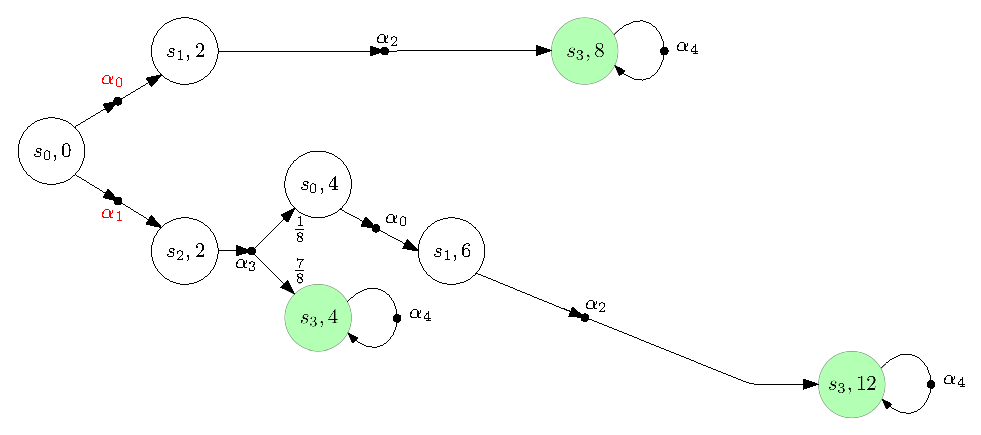
\includegraphics[width=0.8\linewidth]{resources/main-example-unfoldingA}
  \caption{$\mathcal{M}_{\ell_1}$ limited to safe actions of $\mathbb{A}$}
  \label{safe_actions}
\end{figure}
In $\mathcal{M}_{\ell_1}^\mathbb{A}$, we can easily compute the minimal expected cost-to-target for $T_{\ell_1}$ since there is actually only one nondeterministical choice in $\mathcal{M}_{\ell_1}^\mathbb{A}$: either the strategy chooses $\alpha_0$ for the state $(s_0, 0)$ and the expected cost-to-target corresponding to this choice is $8$, or it chooses $\alpha_1$ (we denote this strategy $\sigma^{\alpha_1}$), and the expected cost-to-target is
\[
  \mathbb{E}^{\sigma^{\alpha_1}}_{(s_0, 0)}(\TS^{T_{\ell_1}}) = \frac{7}{8} \cdot 4 + \frac{1}{8} \cdot 12 = 5.
\]
Thus, the minimal expected cost from $s$ to $T$ while ensuring to reach $T$ with probability one is $5 \leq 6$, and thus the \SSPWE{} problem is solved. The optimal pure memoryless strategy $\sigma^{\alpha_1}$ in $\mathcal{M}_{\ell_1}^\mathbb{A}$ corresponds
in $\mathcal{M}$ to the memory strategy trying once $\alpha_1$, and then choosing $\alpha_0$ if it has failed, i.e., trying once a direct sending to the node $n_2$, and then sending the message via the intermediate node $n_1$ if it has failed.
\end{example}

\section{Multi-objective reachability}
\label{most-section}
Now, we interest us in strategies satisfying simultaneously multiple reachability problems \cite{DBLP:journals/lmcs/EtessamiKVY08}.
The problem consisting in deciding the existence of
such a strategy is the \textit{multi-objective stochastic reachability}.
In order to know if we can define a strategy satisfying simultaneously $n$ reachability problems with given probabilities, we interest us in the simultaneously \textit{achievable} vectors $(p_1, \dots, p_n)$ of probabilities for these problems, i.e., such that there exists a strategy ensuring the reachability problem $i$ with a probability $p_i$ for all $i \in \{1, \dots, n\}$.
Furthermore, we interest us in the ``trade-off" curve, named \textit{Pareto curve}, being the set of optimal achievable vectors.
Indeed, there can be some compromises between different reachability properties. For instance,
assume we define a strategy ensuring the reachability to two set of target states $T_1$ and $T_2$ with probabilities $(p_1, p_2)$.
 Modify the strategy to increase the probability $p_1$ of reaching the set $T_1$ may necessitate to lower the probability $p_2$ of reaching the set $T_2$.

\begin{definition}[\textbf{Multi-objective stochastic reachability problem}]
  Let $\mathcal{M}$ be an MDP with state space $S$, action space $A$, and probability transition function $\Delta$, $s \in S$, and $r \in \mathbb{N}$ reachability properties.
  These properties are described by a set of target states $T_i \subseteq S$, and the probability threshold $\alpha_i \in [0, 1] \cap \mathbb{Q}$, for each $i \in \{1, \dots, r\}$.
  The \textit{multi-objective stochastic reachability} problem (\MOSR{}, for short) consists in deciding if there exists a strategy $\sigma$ satisfying
  \[
    \bigwedge_{i=1}^r \mathbb{P}^\sigma_s(\Diamond T_i) \geq \alpha_i.
  \]
\end{definition}

\subsection{Pareto curve}
We now define formally what are achievable vectors for a given \MOSR{} problem and what is the Pareto curve associated.
We actually need these notions to introduce the resolution of all \MOSR{} problems.
Indeed, solving such a problem requires to investigate a multi-objective optimisation problem that is highly linked to this Pareto curve.\\

Let $\mathcal{M}$ be an MDP with state space $S$, action space $A$, and transition probability function $\Delta$, and
$
  \mathcal{Q}_{s, r} := \,?\exists \sigma\; \bigwedge_{i=1}^r \mathbb{P}^\sigma_s(\Diamond T_i) \geq \alpha_i
$
be a \MOSR{} problem for $s \in S$, $r \in \mathbb{N}$, $(T_i)_{i \in \{1, \dots, r\}} \subseteq S^r$, and $\alpha \in ([0, 1] \cap \mathbb{Q})^r$.

\begin{definition}[\textbf{Achievable vectors}]
An \textit{achievable vector of $\mathcal{Q}_{s, r}$} is a vector $(p_i)_{i \in \{1, \dots, r\}}$ such that there exists a strategy $\sigma$ for $\mathcal{M}$ where $p_i = \mathbb{P}^\sigma_s(\Diamond T_i) \geq \alpha_i$ for all $i \in \{1, \dots, r\}$.
Furthermore, the \textit{achievable set of $\mathcal{Q}_{s, r}$} is given by
\[U_{\mathcal{Q}_{s, r}} = \{ \, p \in ([0, 1]) \cap \mathbb{Q})^r \; | \; \exists \sigma, \; p = (\mathbb{P}_s^\sigma (\Diamond T_i))_{i \in \{1, \dots, r\}} \, \}\]
\end{definition}

\begin{definition}[\textbf{Pareto optimal vector}]
  Let $p \in U_{\mathcal{Q}_{s, r}}$ be an achievable vector of $\mathcal{Q}_{s, r}$.
  This vector $p$ is \textit{Pareto optimal} if and only if there does not exists another vector domininating $p$, i.e., $\neg \exists p' \in U_{\mathcal{Q}_{s, r}}$ such that $p \leq p'$ and $p \neq p'$
  (where $\leq$ is the coordinate-wise inequality, i.e., $p\leq p'$ if and only if $p_i \leq p'_i$, for all $i \in \{1, \dots, r\}$).
\end{definition}

\begin{definition}[\textbf{Pareto curve}]
  The \textit{Pareto curve} $\mathpzc{P}_{\mathcal{Q}_{s, r}}$
  of the \MOSR{} problem $\mathcal{Q}_{s, r}$ is the set of Pareto optimal vectors inside $U_{\mathcal{Q}_{s, r}}$, i.e.,
  \[
    \mathpzc{P}_{\mathcal{Q}_{s, r}} =
    \{ p \in U_{\mathcal{Q}_{s, r}} \; | \;
    \neg \exists p'(p' \in U_{\mathcal{Q}_{s, r}} \wedge p \leq p' \wedge p \neq p')\}.
  \]
\end{definition}
For a given \MOSR{} problem, the associated Pareto curve is in general an infinite set.
Actually, this Pareto optimal set is in general a polyhedral set. %\cite{DBLP:journals/lmcs/EtessamiKVY08}.
A way to solve the \MOSR{} would be to enumerate all the vertices of the polytope defining the Pareto curve, or enumerating its facets, but it is not possible to do this in polynomial-time.
However, the Pareto curve can be efficiently approximated with an approximation factor $\epsilon > 0$ \cite{DBLP:conf/focs/PapadimitriouY00}.

\begin{definition}[\textbf{Approximated Pareto curve}]
  Let $\epsilon > 0$, the \textit{$\epsilon$-approximated Pareto curve} of the \MOSR{} problem $\mathcal{Q}_{s, r}$ is the set of achievable vectors $\mathpzc{P}_{\mathcal{Q}_{s, r}}(\epsilon) \subseteq U_{\mathcal{Q}_{s, r}}$ such that, for all achievable vector $p' \in U_{\mathcal{Q}_{s, r}}$, there exists an $\epsilon$-optimal vector $p \in \mathpzc{P}_{\mathcal{Q}_{s, r}}(\epsilon)$
  such that $p' \leq (1 + \epsilon) p$.
\end{definition}

\begin{notation}[\textit{\MOSR{} context}]
When the \MOSR{} problem considered is clear from the context, we use $U$, $\mathpzc{P}$, and $\mathpzc{P}(\epsilon)$ to denote respectively the achievable set, Pareto curve, and $\epsilon$-approximated Pareto curve.
\end{notation}

\subsection{Multi-objective reachability to absorbing targets}

In this subsection, we present an efficient way to solve an \MOSR{} problem for a set of target states only composed of absorbing states. More formally, let $\mathcal{M}=(S, A, \Delta, w, AP, L)$ be an MDP, and
$
  \mathcal{Q}_{s, r} := \,?\exists \sigma\; \bigwedge_{i=1}^r \mathbb{P}^\sigma_s(\Diamond T_i) \geq \alpha_i
$
be a \MOSR{} problem for $s \in S$, $r \in \mathbb{N}$, $(T_i)_{i \in \{1, \dots, r\}} \subseteq S^r$, and $\alpha \in ([0, 1] \cap \mathbb{Q})^r$.
We assume that for all $i \in \{ 1, \dots, r\}$ and for all targets $t \in T_i$, $t$ is absorbing, i.e., there exists an enabled action of $t$, $\alpha \in A(t)$, such that $\Delta(t, \alpha, t) = 1$.\\

In order to solve $\mathcal{Q}_{s, r}$, we need to do some preprocessing on $\mathcal{M}$, to ignore some useless and bad states.
We build a \textit{cleaned up} MDP \sloppy $\mathcal{M}_{clean} = (S_{clean}, A_{clean}, \Delta_{clean}, \Delta_{>0}, w, AP, L)$ from $\mathcal{M}$ and $T = \bigcup_{i \in \{1, \dots, r\}} T_i$ such that
\begin{itemize}
  \item $A_{clean} = A \cup \{\alpha_{dead}\}$,
  \item $S_{clean} = (S \setminus S_{dead}) \cup \{s_{dead}\}$, with
  $S_{dead} = \{s \in S \; | \; \forall \sigma, \; \mathbb{P}_s^\sigma(\Diamond T) = 0\}$
  (remind that this set can be computed efficiently in polynomial time in the size of $\mathcal{M}$ by checking if the vertex representing the state $s$ is connected to $T$ in the underlying graph of $\mathcal{M}$),
  \item we have replaced all \textit{bad states} of $\mathcal{M}$ by the absorbing state $s_{dead}$, i.e., $\forall s, s' \in S_{clean}, \, \forall \alpha \in A_{clean}$, \,
  \[
    \Delta_{clean}(s, \alpha, s') = \begin{cases}
      \sum_{s'' \in S_{dead}} \Delta(s, \alpha, s'') & \text{if } s \neq s' \wedge \, s' = s_{dead}, \\
      1 & \text{if } s=s'=s_{dead} \wedge  \alpha = \alpha_{dead},\\
      0 & \text{if } s=s'=s_{dead} \wedge  \alpha \neq \alpha_{dead}, \\
      \Delta(s, \alpha, s') & \text{otherwise},
    \end{cases}
  \]
  \item $\Delta_{>0}$ is the \textit{safe transition function} defined as follows: let $s, s' \in S_{clean}$, $\alpha \in A_{clean}$,
  \[
    \Delta_{>0}(s, \alpha, s') = \begin{cases}
      1 - \sum_{s'' \in S_{dead}} \Delta(s, \alpha, s'') & \text{if } s \neq s'\, \wedge \, s = s_{dead}, \\
      0 &\text{if } s=s_{dead}, \\
      \Delta_{clean}(s, \alpha, s') &\text{otherwise.}
    \end{cases}
  \]
\end{itemize}

\section{Percentile queries in multi-dimensional Markov decision processes}
In this section, we define some strategies allowing to deal with multiple \textit{percentile queries} in \textit{multi-dimensional Markov decision processes} \cite{DBLP:journals/fmsd/RandourRS17}.
A multi-dimensional MDP is an MDP where the weigth of each action has multiple dimensions.
Remind the \SSPP{} problem in Section \ref{vssp} from Chapter \ref{preliminaries}, consisting in deciding the existence of a strategy satisfying one single percentile query.
We are now interested in defining a strategy solving \textit{simultaneously} multiple \SSPP{} problems on different weight dimensions and for different set of target states.

\begin{definition}[\textbf{Multi-dimensional Markov decision process}]
  A $d$-dimensional MDP is a tuple $\mathcal{M}=(S, A, \Delta, w, AP, L)$ where
  \begin{itemize}
    \item $S, A, \Delta, AP, L$ are defined as for classical MDPs, and
    \item $w$ is a $d$-dimension weight function $w: A \rightarrow \mathbb{N}_0^d$.
    For $k \in \{1, \dots, d\}$, we denote $w_k:A\rightarrow\mathbb{N}_0$ the projection of $w$ on the $k^\text{th}$ dimension, i.e., the function mapping each action $\alpha$ to the $k^\text{th}$ element of the vector $w(\alpha)$.
  \end{itemize}
\end{definition}

\begin{example}[\textit{Multi-dimensional MDP for the wireless sensor network}]
  We update the MDP presented in Example \ref{spg-example} in order to fill in the details left open in the situation described in Example \ref{main-example}.
  \begin{figure}[h]
    \centering
    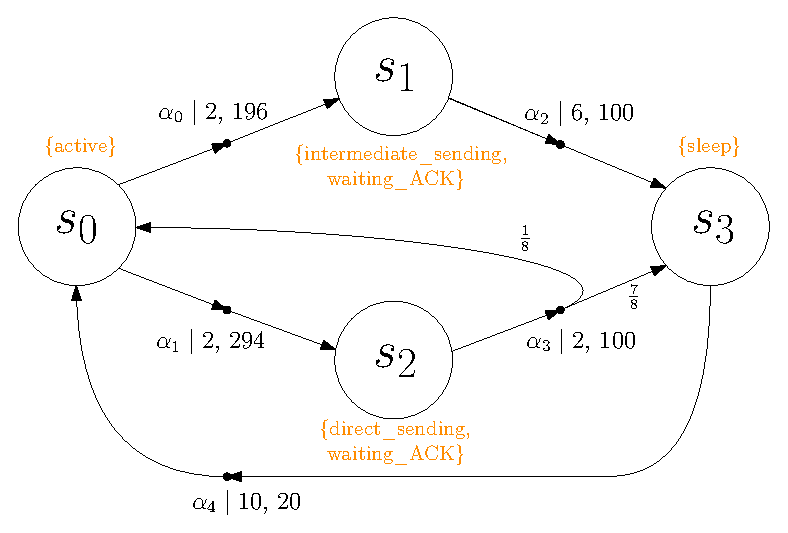
\includegraphics[width=0.6\linewidth]{resources/mdmdp2}
    \captionsetup{justification=centering}
    \caption{Multi-dimensional MDP modelling the situation of Example \ref{main-example}}
    \label{multi-mdp}
  \end{figure}
  We modify the weight function in order to support the energy cost of each action. This modification yields the MDP of Figure \ref{multi-mdp}.
  We assume here that waiting an ACK from a node uses $100$ \textit{mili Joules} ($mJ$), sending a message to $n_1$ uses $196$ $mJ$, sending a message to $n_2$ uses $294$ $mJ$, and staying in the \textit{sleep} state during $10$ $ms$ uses $20$ $mJ$.
\end{example}

\begin{remark}[\textit{Truncated sum in a multi-dimensional MDP}]
  The truncated sum function $\TS$ must be slightly modified in order to handle multidimensional MDPs.
  Indeed, let $\mathcal{M}$ be a $d$-dimensional MDP with state space $S$ and weight function $w$.
  We denote by $\TS^T_{k}$ the truncated sum up to $T$ on the $k^\text{th}$ dimension, with $k \in \{1, \dots, d\}$.
  More formally, let $\pi = s_0 \xrightarrow{\alpha_1} s_1 \xrightarrow{\alpha_2} s_2 \xrightarrow{\alpha_3} \dots \in Paths(s)$ be a path of $\mathcal{M}$ starting from $s \in S$,
  \[
  \TS^T_k(\pi) = \begin{cases}
    \sum_{i=1}^{n} w_k(\alpha_i) & \text{if } \forall i \in \{0, \dots, n-1\}, \, s_{i} \not\in T \, \wedge \, s_n \in T, \\
    + \infty & \text{else}.
  \end{cases}
  \]
  Furthermore, let $\sigma$ be a strategy for $\mathcal{M}$, we can define the event $\Diamond_{k: \, \leq \ell} \, T$ on $\sigma$-paths  starting from $s \in S$ as follows:
  \[
    \Diamond_{k:\,\leq \ell}\,T=\{\pi \in Paths^\sigma(s) \; | \; \TS^T_k(\pi) \leq \ell \}.
  \]
\end{remark}

\begin{definition}[\textbf{\SSPPQ{} problem}]
  Let $\mathcal{M}=(S, A, \Delta, w, AP, L)$ be a $d$-dimensional MDP, $s \in S$, and $q \in \mathbb{N}$ percentile constraints. These percentile constraints are described by a set of target states $T_i \subseteq S$, the dimensions $k_i \in \{1, \dots, d\}$, the cost thresholds $\ell_i \in \mathbb{N}$, and the probability thresholds $\alpha_i \in [0, 1] \cap \mathbb{Q}$, for each $i \in \{1, \dots, q\}$.
  The \textit{stochastic shortest path percentile queries} problem (\SSPPQ{}, for short) consists in deciding if there exists a strategy $\sigma$ such that
  \[
    \bigwedge_{i=1}^r \mathbb{P}^\sigma_s(\Diamond_{k_i:\, \leq \ell_i}\, T_i) \geq \alpha_i.
  \]
\end{definition}

\begin{example}[\textit{\SSPPQ{} problem in the wireless sensor network}] \label{SSPQ-example1}
  Let $\mathcal{M}$ be the MDP of Figure \ref{multi-mdp}, modelling the situation described in Example \ref{main-example} for the node $n_0$.
  We are interested to satisfy multiple percentile queries in $\mathcal{M}$, from the state $s_0$ (i.e., the \textit{active} state of the sensor $n_0$).
  Firstly, we want to ensure with a probability of $80 \%$ that the message will be sent to the sensor $n_2$ and acknowledged within $4 \; ms$ (cf. query $\mathcal{Q}_1$). Secondly, we want to ensure with a probability of $90 \%$ that the message will be sent to the sensor $n_2$ and acknowledged with an energy cost inferior or equal than $700 \; mJ$ (cf. query $\mathcal{Q}_2$).
  \begin{align*}
    &\bigcdot\;\mathcal{Q}_1 := \,  ?\exists \sigma \;\; \mathbb{P}^{\sigma}_{s_0}(\Diamond_{1: \, \leq 4} \, \{s_3\}) \geq 0.8 \\
    &\bigcdot\;\mathcal{Q}_2 := \, ? \exists \sigma \;\; \mathbb{P}_{s_0}^{\sigma}(\Diamond_{2: \, \leq 700} \, \{s_3\}) \geq 0.9
  \end{align*}
  Let $\sigma_1$ and $\sigma_2$ be two pure memoryless strategies for $\mathcal{M}$ such that
  \begin{itemize}
    \item $\sigma_1$ corresponds to the strategy always trying a direct sending to $n_2$, and
    \item $\sigma_2$ corresponds to the strategy sending the message via $n_1$.
  \end{itemize}
  The strategy $\sigma_1$ satisfies $\mathcal{Q}_1$ but does not satisfies $\mathcal{Q}_2$.
  Indeed, this strategy yields %on $Paths^{\sigma_1}(s_0)$
  the events
  \[\Diamond_{1:\, \leq 4}\, \{s_3\} = \Diamond_{2:\, \leq 700}\, \{s_3\} = \{ \pi \in Paths^{\sigma_1}(s_0) \; | \; s_0 %\xrightarrow{\alpha_1}
  s_2 %\xrightarrow{\alpha_3}
  s_3 %\xrightarrow{\alpha_4} \,
  \in Pref(\pi) \},\]
  because $\TS^{\{s_3\}}_1 (s_0 \xrightarrow{\alpha_1}s_2 \xrightarrow{\alpha_3}s_3 \dots) = 4 $,
  $\TS^{\{s_3\}}_2 (s_0 \xrightarrow{\alpha_1}s_2 \xrightarrow{\alpha_3}s_3 \dots) = 394 $, and
  paths of the form $s_0 \xrightarrow{\alpha_1}s_2 \xrightarrow{\alpha_3}s_0 \dots$ necessarily exceed the cost thresholds $4$ and $700$.
  Then, $\mathbb{P}_{s_0}^{\sigma_1}(\Diamond_{1:\, \leq 4}\{s_3\}) = 0.875 \geq 0.8$ and $\mathbb{P}_{s_0}^{\sigma_1}(\Diamond_{2: \, \leq 700} \, \{s_3\}) = 0.875<0.9$.
  In the same way, $\sigma_2$ satisfies $\mathcal{Q}_2$ but does not satisfy $\mathcal{Q}_1$.
  Indeed, $\sigma_2$ yields the events
  \[
    \Diamond_{1:\, \leq 4} \, \{s_3\} = \emptyset, \text{ and }
    \Diamond_{2:\, \leq 700} \, \{s_3\} = \{\pi \in Paths^{\sigma_2}(s_0) \; | \; s_0s_1s_3 \in Pref(\pi)\},
  \]
  because all $\sigma_2$-paths starting from $s_0$ have the form $s_0\xrightarrow{\alpha_0}s_1\xrightarrow{\alpha_2}s_3\dots$,
  $\TS^{\{s_3\}}_1(s_0\xrightarrow{\alpha_0}s_2\xrightarrow{\alpha_2}s_3\dots) = 8 > 4$, and $\TS^{\{s_3\}}_2(s_0\xrightarrow{\alpha_0}s_2\xrightarrow{\alpha_2}s_3 \dots) = 296 \leq 700$. Then,
  $\mathbb{P}_{s_1}^{\sigma_2}(\Diamond_{1:\, \leq 4}\{s_3\}) = 0 < 0.8$ and $\mathbb{P}_{s_0}^{\sigma_2}(\Diamond_{2: \, \leq 700} \, \{s_3\}) = 1 \geq 0.9$.
  \par In order to satisfy both queries at the same
  time, we will consider a finite-memory strategy
  $\sigma_{1\wedge2}$ with two modes, representing
  a \textit{compromise} between these two strategies (cf.
  Figure \ref{strat-compromise}).
  \begin{figure}[h]
    \centering
    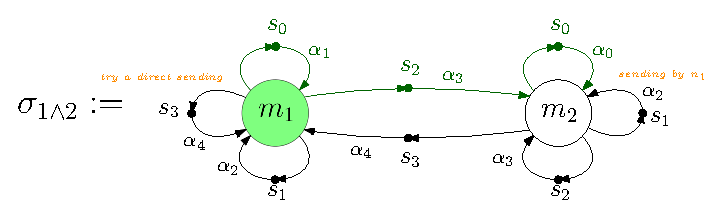
\includegraphics[width=0.7\linewidth]{resources/strategy2}
    \caption{Strategy representing a compromise between $\sigma_1$ and $\sigma_2$ for $\mathcal{M}$}
    \label{strat-compromise}
  \end{figure}
  Indeed, we assume that $\sigma_{1 \wedge 2}$ is initialised in the mode $m_1$ and first try a direct sending to $n_2$. If it fails, it then sends the message via $n_1$.
  As $\sigma_{1 \wedge 2}$ tries a direct sending to $n_2$,
    the cost of this try is $4$ $ms$, $394$ $mJ$ and succeeds with a probability $\frac{7}{8}$.
    If it fails, the strategy next sends the message via $n_1$ and the time threshold is exceeded.
    It does however not matter because the probability threshold to reach $s_3$ within $4$ $ms$ is satisfied. Then, assuming the direct sending has failed, the message is sent via $n_1$. In that case, the total cost of the sending is thus exactly $394 + 296 = 690 < 700$ $mJ$. Thus,
  \begin{itemize}
    \item $\mathbb{P}_{s_0}^{\sigma_{1 \wedge 2}}(\Diamond_{1:\, \leq 4}\, \{s_3\}) = 0.875 \geq 0.8 \implies \sigma_{1 \wedge 2} \text{ satisfies }\mathcal{Q}_1, \text{ and}$
    \item $\mathbb{P}_{s_0}^{\sigma_{1 \wedge 2}}(\Diamond_{2:\, \leq 700}\, \{s_3\}) = 1 \geq 0.9 \implies \sigma_{1 \wedge 2} \text{ satisfies }\mathcal{Q}_2.$
  \end{itemize}

Assume now that we want to additionally ensure that the message will be sent and acknowledged within $8$ $ms$ with a probability of $0.9$.
That yields the following \SSPPQ{} problem:
\[
  ?\exists \sigma \;\; \mathbb{P}^{\sigma}_{s_0}(\Diamond_{1: \, \leq 4} \, \{s_3\}) \geq 0.8 \; \wedge \;
   \mathbb{P}^{\sigma}_{s_0}(\Diamond_{1: \, \leq 8} \, \{s_3\}) \geq 0.9 \; \wedge \;
  \mathbb{P}_{s_0}^{\sigma}(\Diamond_{2: \, \leq 700} \, \{s_3\}) \geq 0.9
\]
None pure strategy can satisfy simultaneously these percentile queries, even finite-memory strategies.
In order to satisfy this \SSPPQ{} problem, we additionally need the notion of randomisation in our strategies (cf. ).
\end{example}

\begin{definition}[\textbf{Randomised finite-memory strategies}]
  Let \sloppy $\mathcal{M}={(S, A, \Delta, w, AP, L)}$ be an MDP. A \textit{finite-memory randomised strategy} $\sigma = (Q, \sigma_\alpha, \delta, \delta_0)$ is a \textit{stochastic Moore machine}, where
  \begin{itemize}
    %\item $Q, \delta, \delta_0$ are defined the same way as for pure finite-memory strategies, and
    \item $Q$ is a finite set of \textit{modes},
    \item $\sigma_\alpha: Q \times S \rightarrow \mathcal{D}(A)$ is the \textit{stochastic next action function} giving, for each $s \in S$, a probability distribution on actions of $A(s)$ following a mode $q \in Q$ in which the machine is currently,
    \item $\delta: Q \times S \rightarrow \mathcal{D}(Q)$ is the \textit{stochastic transition function},
    \item $\delta_0: S \rightarrow Q$ is the \textit{initialisation function}, defined as for the pure strategy, giving the initial mode $q \in Q$, following a state $s \in S$ from which the machine is initialised.
  \end{itemize}
\end{definition}

According to this definition, the probability distribution defined on the successors of each state $s$ of a Markov chain induced by such a strategy additionally depends on the probability distribution defined on enabled actions of $s$ given by the stochastic next action function as well as the probability distribution defined on modes of the Moore Machine given by the stochastic transition function.

\begin{definition}[\textbf{Markov chain induced by a randomised finite-memory strategy}]
  Let $\mathcal{M}=(S, A, \Delta, w, AP, L)$ be an MDP and $\sigma=(Q, \sigma_\alpha, \delta, \delta_0)$ be a randomised finite-memory strategy for $\mathcal{M}$.
  The product of $\mathcal{M}$ by $\sigma$ is given by
  \[
    \mathcal{M} \times \sigma = \mathcal{M}^\sigma = (S \times Q, \Delta^\sigma, AP, L^\sigma)
  \]
  where $\mathcal{M}^\sigma$ is the MC induced by the randomised finite-memory strategy $\sigma$ and where, for all states $s, s' \in S$, and for all modes $q, q' \in Q$,
  \begin{itemize}
    \item $\Delta^\sigma((s, q), (s', q')) =
    \delta(q, s)(q') \cdot \sum_{\alpha \in A(s)} \sigma_\alpha(q, s)(\alpha) \cdot \Delta(s, \alpha, s')$
    \item $L^\sigma(s, q) = L(s)$.
  \end{itemize}
\end{definition}

\begin{remark}[\textit{Weight function in an MC induced by a randomised strategy}]
  We do not consider the weight function of any induced MC by a randomised strategy $\sigma$ in this context.
  Indeed, the weight of a transition depends on the action chosen by the strategy. Here, as actions are chosen randomly following a probability distribution defined on enabled actions of each state, this information is lost in the induced MC.
  It is however possible to define a weight function
  \[
    \overline{w}^\sigma: (S \times Q)^2 \rightarrow \mathbb{Q}_{>0}, \; ((s, q), (s', q')) \mapsto \delta(q, s)(q') \cdot \sum_{\alpha \in A(s)} \sigma_{\alpha}(q, s)(\alpha) \cdot w(\alpha),
  \]
  referring to the expected weight of each transition in the induced MC, but this definition is irrelevant in our context.
\end{remark}

As for pure strategy, there exists a subset of randomised finite-memory strategies with only one mode for a given MDP.
These randomised strategies are \textit{memoryless}.

\begin{definition}[\textbf{Randomised memoryless strategy}]
  Let $\mathcal{M}=(S, A, \Delta, w, AP, L)$ be an MDP. A randomised memoryless strategy $\sigma$ is a function
  $
    \sigma: S \rightarrow \mathcal{D}(A),
  $ given, following a state $s \in S$, a probability distribution defined on the enabled action of $s$.
\end{definition}

Let $\mathcal{M}=(S, A, \Delta, w, AP, L)$ be a $d$-dimensional MDP,
$s^* \in S$, and $q \in \mathbb{N}$ percentile constraints described by
$T_i \subseteq S$, the dimension $k_i \in \{1, \dots, d\}$, the cost threshold $\ell_i \in \mathbb{N}$, and the probability threshold $\alpha_i \in [0, 1] \cap \mathbb{Q}$, for each constraints $i \in \{1, \dots, q\}$.
We will now introduce an algorithm to solve the \SSPPQ{} problem for the state $s^*$ and these $q$ constraints. This algorithm allows to build an optimal strategy with both finite-memory and randomisation to satisfy the problem.
Note that we assume all dimensions of $\mathcal{M}$ being relevant for this problem, i.e., $\bigcup_{i \in \{1, \dots q\}} k_i = \{1, \dots, d\}$.
On the other hand, we simply drop the $n$ irrelevant dimensions of $\mathcal{M}$ for the problem and we only consider the $d-n$ remaining one.
In order to describe this algorithm, we need to define the \textit{multi-dimensional unfolding of an MDP}.

\begin{definition}[\textbf{Multi-dimensional unfolding of an MDP}]
The \textit{$d$-dimensional unfolding of the MDP $\mathcal{M}$ from the state $s^*$
up to the highest cost threshold of $(\ell_i)_{i \in \{1, \dots, q\}}$ on each dimension of $(k_i)_{i \in \{1, \dots, q\}}$} is a $1$-dimensional MDP \sloppy $\mathcal{M}' = {(S', A', \Delta', AP, L')}$ defined as follows:
  \begin{itemize}
    \item $S'$ is composed of states $(s, v_1, \dots, v_d)$ such that $s \in S$ and, for each dimension $k \in \{1, \dots, d\}$, $v_k \in \{0, \dots, \ell^{\max}_k\} \cup \{\bot\}$, where $\ell^{\max}_k$ is the maximum threshold on the dimension $k$, i.e., \[\ell^{\max}_k = \max_{i \in \{1, \dots, q\} \; | \; k_i = k }  \, \ell_i,\]
    and we consider that $\bot > l$
    and $\bot + v = \bot$, for all $v \in \mathbb{N}$.
    Intuitively, the vector $(v_1, \dots, v_d)$ records the cost of paths on all the dimensions while unfolding $\mathcal{M}$.
    Furthermore, as we unfold $\mathcal{M}$ from $s^*$, we have
    $(s^*, 0, \dots, 0) \in S'$, and $(s, 0, \dots, 0) \not\in S'$ for all states $s \neq s^*$.
    \item $A'$ is the set of action of the unfolding such that $\alpha \in A'$
    for all action $\alpha \in A$, and
    $A'(s, v_1, \dots, v_d) = A(s)$
    for all $(s, v_1, \dots, v_d) \in S'$.
    \item $\Delta'$ is the probability transition function defined as follows: let $x = (s, v_1, \dots, v_d) , \, x'=(s', v'_1, \dots, v'_d) \in S'$, $\alpha \in A'(s)$,
    and
    $succ_k: S' \times A' \rightarrow \{0, \dots, \ell^{\max}_k\},$
    \[((s, v_1, \dots, v_d), \, \alpha) \mapsto \begin{cases}
      v_k + w_k(\alpha) & \text{if } v_k + w_k(\alpha) \leq \ell^{\max}_k \\
      \bot & \text{else},
    \end{cases}\]
    referring to the $\alpha$-successor of $(s, v_1, \dots, v_d)$ on the cost dimension $k \in \{1, \dots, d\}$,
    \[
    \Delta'(x, \alpha, x') = \begin{cases}
      \Delta(s, \alpha, s') & \text{if } \forall k \in \{1, \dots, d\}, \, v'_k = succ_k(x) \\
      & \quad \text{and }\exists k \in \{1, \dots, d\}, \, v_k \neq \bot, \\
      \sum_{s'' \in S} \Delta(s, \alpha, s'')
      & \text{if } \forall k \in \{1, \dots, d\},\, succ_k(x) = \bot \\
      & \quad \text{and } x \neq x', \, x' = s_\bot,\\
      1 & \text{if } x=x'=s_\bot \text{ and } \alpha = \alpha_\bot, \\
      0 & \text{otherwise,}
    \end{cases}
    \]
    where $s_\bot$ represents the state for which the cost thresholds have been exceeded on all the dimensions, i.e., where for all $k \in \{1, \dots, d\}$, $v_k = \bot$. We consider that this state has only one enabled action $\alpha_\bot$.
    \item $L': S' \rightarrow AP,\, (s, v_1, \dots, v_d) \mapsto L(s)$ is the labelling function of the unfolding.
  \end{itemize}
\end{definition}

This definition allows us to describe an algorithm defined to solve the \SSPPQ{} problem for the state $s^*$ and the $q$ constraints described above:

\begin{algorithm}
\caption{Solving the \SSPPQ{} problem}\label{ssppq-algo}
\begin{enumerate}
\item We build the MDP $\mathcal{M}'$, being the $d$-dimensional unfolding of $\mathcal{M}$ up to the highest cost thresholds on each of these dimensions.
  A path is thus discarded only if its current cost exceeds all highest threshold on each of these dimensions.
  Indeed, some paths exceeding the cost threshold of a request could still interesting to satisfy the others.
  \item Then, we compute the set of target states \[T'_i = \{ (s, v_1, \dots, v_d) \in S' \; | \; s \in T_i  \; \wedge \; v_{k_i} \leq l_i \}\] in $\mathcal{M}'$ for each request $i \in \{1, \dots, q\}$.
  \item Finally, we are left with a \MOSR{} problem on $\mathcal{M}'$: we are looking for a strategy ensuring that each of these sets $T'_i$ are reached from $(s^*, 0, \dots, 0)$ with a probability $\alpha_i$ (cf. Section \ref{mosr-section}).
\end{enumerate}
\end{algorithm}

\begin{theorem}[\textit{\textbf{Solving the \SSPPQ{} problem}}]
  The \SSPPQ{} problem can be decided in exponential time in general, and pseudo-polynomial time for simultaneously single-dimension and single-target queries.
  Randomised exponential-memory strategies are always sufficient and in general necessary.
  A satisfying strategy can be built in exponential time.
\end{theorem}

\begin{example}[\textit{Complex \SSPPQ{} problem in the wireless sensor network}]
  We apply the algorithm \ref{ssppq-algo} to answer to the percentile request left open in Example \ref{SSPQ-example1}:
  \[
  ?\exists \sigma \;\; \underbrace{\mathbb{P}^{\sigma}_{s_0}(\Diamond_{1: \, \leq 4} \, \{s_3\}) \geq 0.8}_{\mathcal{Q}_1} \; \wedge \;
   \underbrace{\mathbb{P}^{\sigma}_{s_0}(\Diamond_{1: \, \leq 8} \, \{s_3\}) \geq 0.9}_{\mathcal{Q}_2} \; \wedge \;
  \underbrace{\mathbb{P}_{s_0}^{\sigma}(\Diamond_{2: \, \leq 700} \, \{s_3\}) \geq 0.9}_{\mathcal{Q}_3}
  \]
  In order to solve this \SSPPQ{} problem, we build the $2$-dimensional unfolding $\mathcal{M'}$ of the MDP of Figure \ref{multi-mdp}, for the state $s_0$, the cost thresholds $\ell_1 = 4$, $\ell_2 = 8$, $\ell_3 = 700$, and the dimensions $k_1 = k_2 = 1$, $k_3 = 2$ (cf. Figure \ref{multi-unfolding}).
  \begin{figure}[h]
    \centering
    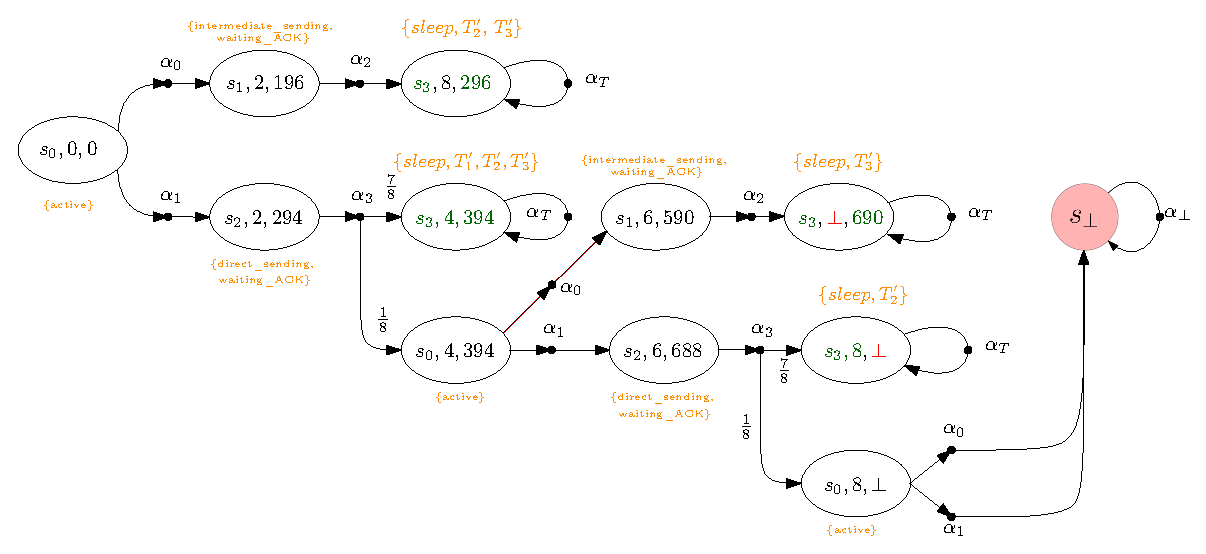
\includegraphics[width=\linewidth]{resources/SSP-PQ-unfolding}
    \captionsetup{justification=centering}
    \caption{Unfolding of the MDP of Figure \ref{multi-mdp} from $s_0$ up to the cost thresholds $4, \, 8$ on the time dimension, and $700$ on the energy dimension}
    \label{multi-unfolding}
  \end{figure}
  As each constraint describes a percentile problem,
  and as the set of target states for all constraints is $\{s_3\}$, we do not need to consider states after that $\{s_3\}$ is reached in all paths starting from $(s_0, 0, 0)$ in $\mathcal{M}'$.
  We can thus make all states referring to $s_3$  absorbing in $\mathcal{M}'$.
  The new sets of target states are $T'_1 = \{(s_3, 4, 394)\}$, $T'_2 = \{(s_3, 8, 296), \, (s_3, 4, 394), \, (s_3, 8, \bot)\}, \, T'_3 = \{ (s_3, 8, 296), \, (s_3, 4, 494) \}$
  for all query $\mathcal{Q}_i$, with $i \in \{1, \dots, 3\}$. As all target states are absorbing, we can build a satisfying randomised memoryless optimal strategy in polynomial time in the size of $\mathcal{M}'$.
  %The randomised memoryless strategy $\sigma$ such that $\sigma(s')(\alpha) = 1$ for all $s' \in S'$ such that $\alpha \in A(s)$, $|A(s)| = 1$, and
  %$\sigma((s, 0, 0))(\alpha_1) = 1$, $\sigma((s_0, 4, 394))(\alpha_0) = \sigma((s_0, 4, 394))(\alpha_1) = \frac{1}{2}$ satisfies the problem.
  We build the randomised memoryless strategy
  \[
  \sigma(s')(\alpha) = \begin{cases}
    1 & \text{if } \alpha \in A(s) \text{ and } |A(s)| = 1,
    \text{ or } s'=(s_0, 0, 0), \, \alpha=\alpha_1, \\
    \frac{1}{2} & \text{if } s'=(s_0,4,394) \text{ and } \alpha \in \{\alpha_0, \alpha_1\},\\
    0 & \text{otherwise}.
  \end{cases}
  \]
  The MC induced by $\sigma$ is given on Figure \ref{mc-unfolding}.
  \begin{figure}[h]
    \centering
    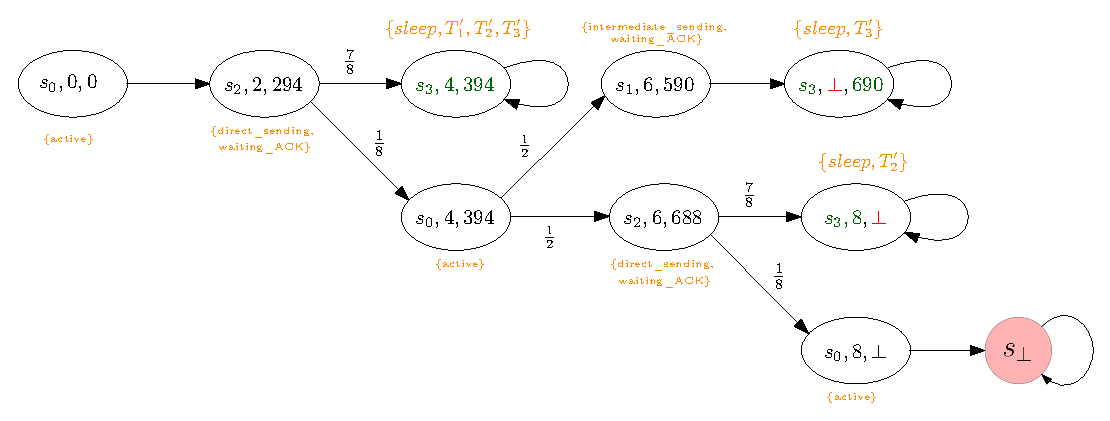
\includegraphics[width=\linewidth]{resources/SSP-PQ-unfolding2}
    \caption{Product of $\sigma$ with $\mathcal{M}'$, yielding the induced MC by $\sigma$}
    \label{mc-unfolding}
  \end{figure}
  We have $\mathbb{P}^\sigma_{(s_0, 0, 0)}(\Diamond T'_1) = \frac{7}{8}$, $\mathbb{P}^\sigma_{(s_0, 0, 0)}(\Diamond T'_2) = \frac{7}{8} + \frac{1}{8} \cdot \frac{1}{2} \cdot \frac{7}{8} \geq 0.9$, and
  $\mathbb{P}^\sigma_{(s_0, 0, 0)}(\Diamond T'_3) = \frac{7}{8} + \frac{1}{8} \cdot \frac{1}{2} \geq 0.9$. Thus, we have that $\sigma$ satisfies $\mathcal{Q}_1$, $\mathcal{Q}_2$, and $\mathcal{Q}_3$.
  The strategy $\sigma$ is memoryless in $\mathcal{M}'$, and exponential-memory in $\mathcal{M}$.
  Thus, the \SSPPQ{} problem is solved.
\end{example}
